\begin{center}
 \textsc{Физбой, 7--8 классы.}
\end{center}
\vspace{0.01cm}
\hrule
\parindent=0mm

\task{Легкая пружина длины $l$, жесткости $k$ установлена на столе
  вертикально. На нее падает небольшой шарик массой $m$. Определите,
  на какой высоте $h$ от поверхности стола шарик будет иметь
  максимальную скорость.}

\task{На пробку массой $m_{\mbox{\textit{пр}}}$ намотана проволока из
  алюминия. Плотность пробки равна $\rho_{\mbox{\textit{пр}}} =
  0{,}5\cdot10^3\mbox{ кг/м}^3$, алюминия $\rho_{\mbox{\textit{ал}}} =
  2{,}7\cdot10^3\mbox{ кг/м}^3$, воды $\rho_{\mbox{\textit{в}}} =
  1\cdot10^3\mbox{ кг/м}^3$. Определите, какую минимальную массу
  $m_{\mbox{\textit{ал}}}$ проволоки надо намотать на пробку, чтобы
  пробка вместе с проволокой полностью погрузилась в воду.}

\taskpic{К концу однородной палочки массой $M = 4{,}4\mbox{ г}$
  подвешен на невесомой нити однородный алюминиевый шарик радиуса $r =
  0{,}5\mbox{ см}$. Палочку кладут на край стакана с водой, добиваясь
  такого положения равновесия, при котором погруженной в воду окажется
  половина шарика. Плотность алюминия равна $\rho_{\mbox{\textit{ал}}}
  = 2{,}7\cdot10^3\mbox{ кг/м}^3$, плотность воды
  $\rho_{\mbox{\textit{в}}} = 1\cdot10^3\mbox{ кг/м}^3$. Определите, в
  каком отношении $y/x$ делится длина палочки в этом случае. Объем
  шара радиуса $r$ равен $4\pi
  r^3/3$.}{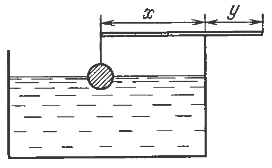
\includegraphics[width=4cm]{fbs03.png}}

\taskpic{На пустую катушку магнитофона, делающую одинаковое количество
  оборотов в единицу времени, перематывается магнитная лента. После
  перемотки конечный радиус $r_{\mbox{\textit{к}}}$ намотки оказался в
  семь раз больше начального радиуса $r_{\mbox{\textit{н}}}$. Время
  перемотки ленты равно $t_1$. За какое время $t_2$ на катушку
  перемотается лента такой же длины, но вдвое более
  тонкая?}{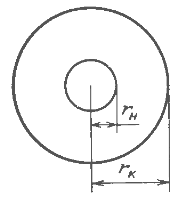
\includegraphics[width=3cm]{fbs04.png}}

\taskpic{Записывая свои воспоминания, барон Мюнхаузен засиделся до
  поздней ночи при свечах. Обе свечи одинаковой длины $l$ он зажег
  одновременно и поставил, как показано на рисунке. Скоро он заметил,
  что тень первой свечи на левой стене неподвижна, а тень второй свечи
  на правой стене укорачивается со скоростью $v$. Через какое время
  барон останется в полной темноте? Считайте, что
  $d_1=d_2=d_3$.}{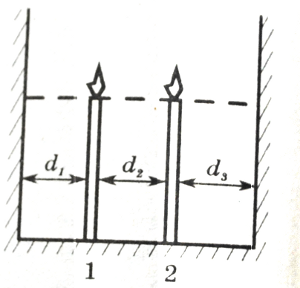
\includegraphics[width=4cm]{fbs05.png}}

\task{Автомобиль проехал половину пути со скоростью $v_1 = 60\mbox{
    км/ч}$. Половину оставшегося времени движения он ехал со скоростью
  $v_2 = 15\mbox{ км/ч}$, а последний участок пути --- со скоростью
  $v_3 = 45\mbox{ км/ч}$. Чему равна средняя скорость автомобиля на
  всем пути?}

\setcounter{notask}{1}